\refstepcounter{section}
\section*{Lecture 12: Towards the action for Gravity: Invariant Volumes}
\addcontentsline{toc}{section}{Lecture 12: Towards the action for Gravity: Invariant Volumes}
Motion under gravity can be determined once we know the metric $g_{\mu\nu}$, however, we want to see how to obtain the equation for the metric. In other words, since equations of motion can be derived from \textit{action}, we need to find an action for gravity!
\subsection{Maxwell's action in spacetime}
In free space, the \textit{electromagnetic} action can be written as:
$$\Ss_{\mathrm{EM}} = \int \dd^4\fvec{x} \qty[-\frac{1}{4\mu_0}F_{\mu\nu}F^{\mu\nu}]$$
Here $F_{\mu\nu}$ is the anti-symmetric electromagnetic tensor and is defined by:
\begin{equation}\label{eqn:fmunu}
    F_{\mu\nu}:= \partial_\mu A_{\nu} - \partial_\nu A_{\mu}\qquad F_{\mu\nu} = -F_{\nu\mu}
\end{equation}
$A^\mu = \qty(\phi, \tvec{A})$ is the four-potential, which we will simply call the \textit{electromagnetic field}. From the above defined action, we can obtain all of Maxwell's equations. We can manipulate the action as follows,
\begin{align*}
    \Ss_{\mathrm{EM}} &= \frac{1}{4\mu_0}\int \dd^4\fvec{x} - \qty[\partial_\mu A_\nu -\partial_\nu A_\mu  ]F^{\mu\nu}\\
    &=2\times \frac{1}{4\mu_0}\int \dd^4\fvec{x} \qty[-\partial_\mu A_{\nu}F^{\mu\nu}]\qquad \text{(using anti-symmetric property)} \\
    &\myeq{IBP}\frac{1}{2\mu_0}\int \dvol \qty[A_\nu \partial_\mu F^{\mu\nu} - \partial_\mu\qty(A_\nu F^{\mu\nu})]
\end{align*} 
The last integral is a total-derivative which can be converted to the surface integral using Stokes' theorem. We assume that at spatial and temporal infinities, the fields vanish and thus, the integral is zero. Then we obtain,
\begin{align*}
    \Ss_{\mathrm{EM}} = \frac{1}{2\mu_0}\int \dvol \qty[A_\nu \partial_\mu F^{\mu\nu}] =\frac{1}{2\mu_0}\int \dvol \qty[A_\nu \partial_\mu \qty(\partial_\mu A_{\nu} - \partial_\nu A_{\mu}) ] 
\end{align*}
\textbf{Properties of the Maxwell action:}
\begin{itemize}
    \item $\Ss_{\mathrm{EM}}$ is a functional of $A_\mu$, that is, it takes a value of $A_\mu$ and returns a number.
    \item $\Ss_{\mathrm{EM}}$ is a scalar under Lorentz transformation. We can see this since the indices in $F$ are contracted and $\dvol$ can be shown to be Lorentz-invariant. 
    \item $\Ss_{\mathrm{EM}}$ has atmost two derivatives of the field $A_\mu$
\end{itemize}
Einstein took inspiration from this action, however, he tried to include the invariance of this action for general transformations too! He proposed that \textit{action} for the metric should be of the following form:
$$\Ss_{\mathrm{G}} = \int \dvol f\qty(g_{\mu\nu}, \partial_\alpha\partial_\beta g_{\mu\nu})$$
The above mentioned form has many subtleties, let us look at them one by one. First note that if the function $f$ has to be a scalar under general coordinate transformations, then the integral measure $\dvol$ must also be a scalar. However, this is not apriori obvious. As an example, note how the `volume' element changes when we move from Cartesian to polar coordinates. 
\begin{figure}[H]
    \centering
    

\tikzset{every picture/.style={line width=0.75pt}} %set default line width to 0.75pt        

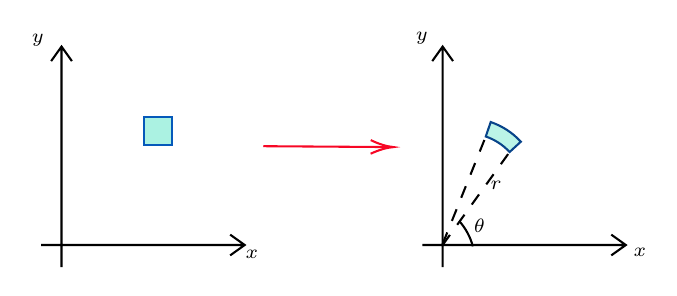
\begin{tikzpicture}[x=0.75pt,y=0.75pt,yscale=-1,xscale=1]
%uncomment if require: \path (0,180); %set diagram left start at 0, and has height of 180

%Shape: Axis 2D [id:dp02539055479397534] 
\draw  (72,137.61) -- (170.06,137.61)(81.81,42) -- (81.81,148.23) (163.06,132.61) -- (170.06,137.61) -- (163.06,142.61) (76.81,49) -- (81.81,42) -- (86.81,49)  ;
%Shape: Axis 2D [id:dp12109142679695195] 
\draw  (255.62,137.61) -- (353.68,137.61)(265.43,42) -- (265.43,148.23) (346.68,132.61) -- (353.68,137.61) -- (346.68,142.61) (260.43,49) -- (265.43,42) -- (270.43,49)  ;
%Straight Lines [id:da7218148845298954] 
\draw [color={rgb, 255:red, 247; green, 7; blue, 37 }  ,draw opacity=1 ]   (179,90) -- (239.68,90.42) ;
\draw [shift={(241.68,90.43)}, rotate = 180.4] [color={rgb, 255:red, 247; green, 7; blue, 37 }  ,draw opacity=1 ][line width=0.75]    (10.93,-3.29) .. controls (6.95,-1.4) and (3.31,-0.3) .. (0,0) .. controls (3.31,0.3) and (6.95,1.4) .. (10.93,3.29)   ;
%Shape: Square [id:dp07048562368847666] 
\draw  [color={rgb, 255:red, 5; green, 89; blue, 186 }  ,draw opacity=1 ][fill={rgb, 255:red, 80; green, 227; blue, 194 }  ,fill opacity=0.48 ] (121.57,76) -- (135,76) -- (135,89.43) -- (121.57,89.43) -- cycle ;
%Straight Lines [id:da8832243520760285] 
\draw  [dash pattern={on 4.5pt off 4.5pt}]  (265.43,137.12) -- (286.21,85.34) ;
%Straight Lines [id:da5448388205855526] 
\draw  [dash pattern={on 4.5pt off 4.5pt}]  (265.43,137.61) -- (297.68,92.82) ;
%Shape: Block Arc [id:dp5133838655063991] 
\draw  [color={rgb, 255:red, 8; green, 68; blue, 138 }  ,draw opacity=1 ][fill={rgb, 255:red, 80; green, 227; blue, 194 }  ,fill opacity=0.39 ] (288.58,78.37) .. controls (294.03,80.22) and (299.05,83.41) .. (303.1,87.84) -- (297.68,92.82) .. controls (294.48,89.32) and (290.51,86.8) .. (286.21,85.34) -- cycle ;
%Shape: Arc [id:dp4876255611960163] 
\draw  [draw opacity=0] (273.47,126.12) .. controls (276.65,129.72) and (278.82,133.88) .. (279.98,138.24) -- (251,146) -- cycle ; \draw   (273.47,126.12) .. controls (276.65,129.72) and (278.82,133.88) .. (279.98,138.24) ;  

% Text Node
\draw (169,138.4) node [anchor=north west][inner sep=0.75pt]  [font=\scriptsize]  {$x$};
% Text Node
\draw (66,34.4) node [anchor=north west][inner sep=0.75pt]  [font=\scriptsize]  {$y$};
% Text Node
\draw (356,137.4) node [anchor=north west][inner sep=0.75pt]  [font=\scriptsize]  {$x$};
% Text Node
\draw (251,33.4) node [anchor=north west][inner sep=0.75pt]  [font=\scriptsize]  {$y$};
% Text Node
\draw (287,105.4) node [anchor=north west][inner sep=0.75pt]  [font=\scriptsize]  {$r$};
% Text Node
\draw (279,123.4) node [anchor=north west][inner sep=0.75pt]  [font=\scriptsize]  {$\theta $};


\end{tikzpicture}

\end{figure}
\noindent
In Cartesian coordinates, the volume element (actually the area element since it is 2D) is $\dd V = \dd x \ \dd y$ while in the polar coordinates, the volume elements is $\dd V' = \dd r \ (r\ \dd \theta) = r \ \dd \theta \ \dd r$
There is an extra factor $r$ apart from the coordinate differential. We denote it by $J(r,\theta)$ which is the \textit{Jacobian} of the transformation. Thus, to keep the volume element invariant, we need to add the effect of the Jacobian too!
\subsection{Metric, Transformations and Jacobian}
Consider the Leibniz formula for the determinant of a square $n\times n$ matrix. The formula says that for any matrix A, we have \footnote{You may also look into Sec 6.5.3 \href{https://raw.githubusercontent.com/LoneWolf1304/Notes/main/Tensor Analysis/main.pdf}{here}!}:
$$\det(A) = \sum_{\tau \in S_n} \operatorname{sgn}(\tau) \prod_{i=1}^{n} a^{i}_{\tau(i)} 
= \sum_{\sigma \in S_n} \operatorname{sgn}(\sigma) \prod_{i=1}^{n} a_{\sigma(i)}^{i}$$ 
From this, we can derive another formula for the determinant using the Levi-Civita symbol:
\begin{identity}
$$\det(M)= \widetilde{\upepsilon}^{\mu_1'\ldots \mu_n'} \widetilde{\upepsilon}_{\mu_1\ldots \mu_n} \tensor{A}{^{\mu_1} _{\mu_1'}}\tensor{A}{^{\mu_2} _{\mu_2'}}\ldots\tensor{A}{^{\mu_n} _{\mu_n'}}$$
\end{identity}
Let us keep this aside and calculate the volume element for a two-dimensional coordinate system, in primed and unprimed frames. Note that the volume element can be written in the following way: \begin{align*}
    \dd V &= J(\fvec{x}) \frac{1}{2!}\upepsilon_{\alpha\beta}(-1)^p \dd x^\alpha \dd x^\beta\\
    \dd V &= J(\fvec{x}') \frac{1}{2!}\upepsilon_{\mu\nu}(-1)^p \dd x^\mu \dd x^\nu
\end{align*}
What just happened here! \emoji{woozy-face}. First note that $p$ here is the sign of the permutation, that is, if the permutation $\alpha,\beta$ is odd then $p=-1$, else $p=0$. This is done to ensure that the quantity is positive. Also note that, $J$ as defined here should always be taken to be positive, to make $\dd V$ non-negative. Subtleties aside, if we expand the first expression, we would get:
$$\dd V = J(\fvec{x}) \frac{1}{2}\qty(\upepsilon_{12} (-1)^0 \dd x^1 \dd x^2 + \upepsilon_{21}(-1)^{1} \dd x^2 \dd x^{1})= J(\fvec{x})\dd x^1 \dd x^2 $$
This is indeed the expression for the volume element in the unprimed frame. The above formula is related to differential forms and wedge products which are defined in terms of \textit{alternating-operator} and gives a generalisation of the volume element $\dd V = dx^1\wedge dx^2 \wedge \ldots$ which we will not explore.\\[0.2cm]
Anyways, let us now calculate something. Since we want $\dd V = \dd V'$, then we demand that:
\begin{align*}
    J(\fvec{x})\frac{1}{2!} \upepsilon_{\alpha\beta}(-1)^p \dd x^\alpha \dd x^\beta &= J(\fvec{x}') \frac{1}{2!} \upepsilon_{\mu\nu}(-1)^p \dd x'^\mu \dd x'^\nu
\end{align*}
Let us take the primed coordinate to be Cartesian and hence, $J(\fvec{x}') =1$. Then, transforming the coordinates we obtain:
\begin{align*}
    J(\fvec{x})\frac{1}{2!} \upepsilon_{\alpha\beta}(-1)^p \dd x^\alpha \dd x^\beta &= \frac{1}{2!} \upepsilon_{\mu\nu}(-1)^p \trmat{\mu}{\alpha}\trmat{\nu}{\beta}\dd x^\alpha \dd x^\beta
\end{align*}
Now, since the differentials are arbitrary, both quantities are equal. Let us contract both sides with $\upepsilon^{\alpha\beta}$ which gives us:
$$J(\fvec{x}) \frac{1}{2!} \upepsilon_{\alpha\beta}\upepsilon^{\alpha\beta} = \frac{1}{2!}\upepsilon_{\mu\nu}\upepsilon^{\alpha\beta}\trmat{\mu}{\alpha}\trmat{\nu}{\beta}=\det(\trmat{\mu}{\alpha})$$
In the RHS, we have used the formula that we had written for the determinant previously. In the LHS, note that $\upepsilon_{\alpha\beta}\upepsilon^{\alpha\beta} $ will be $2$ and hence, the final result that we obtained is:
$$J(\fvec{x}) = \det(\trmat{\mu}{\alpha})$$
Thus, the Jacobian of the transformation is basically the determinant of the transformation matrix. Using the above found expression, we can write the volume element (now, in arbitrary dimensions) as:
$$\dd V = \det(\trmat{\mu}{\nu}) \prod\limits_{\alpha}\dd x^\alpha $$
Now, let us take the metric. Since the primed frame is \textit{flat}, the metric there is Minkowski, $\eta_{\mu\nu}$. Then, from the transformation rule, we will have:
$$g = \Lambda^{\mathrm{T}}\eta \Lambda$$
Since the determinant of $\Lambda$ and $\Lambda^{\mathrm{T}}$ are same and $\det(\eta)=-1$, we obtain:
$$\det(g) = -\det(\Lambda)^2 = -J^2 \implies J = \sqrt{|-\mathfrak{g}|}$$
where we have defined $\mathfrak{g}:= \det(g)$, the determinant of the metric tensor for the space. Generalising to $n$ dimensions, we have the volume element as:
$$\dd V = \dd^n \vec{x} \ \sqrt{|-\mathfrak{g}|}$$
As an example, for 2D polar coordinates, we have: $$g\equiv  \mathrm{diag}(1, r^2)\implies \mathfrak{g} = r^2 \implies \dd V = \dd r \ \dd \theta \ \sqrt{r^2} =r \ \dd r\ \dd \theta$$ And for 3D  spherical coordinates we have, $$g\equiv  \mathrm{diag}(1, r^2, r^2\sin^2\theta)\mathfrak{g} = r^4\sin^2\theta \implies \dd V = \dd r \ \dd \theta\ \dd \phi \ \sqrt{r^4\sin^2\theta} =r^2 \sin\theta\ \dd r \ \dd \theta\ \dd \phi $$
which are indeed the case as we know from our experience! Thus, this gives a nice expression to deal with the volume elements in some arbitrary space with some arbitrary metric. 